\begin{figure}[ht]
    \centering
    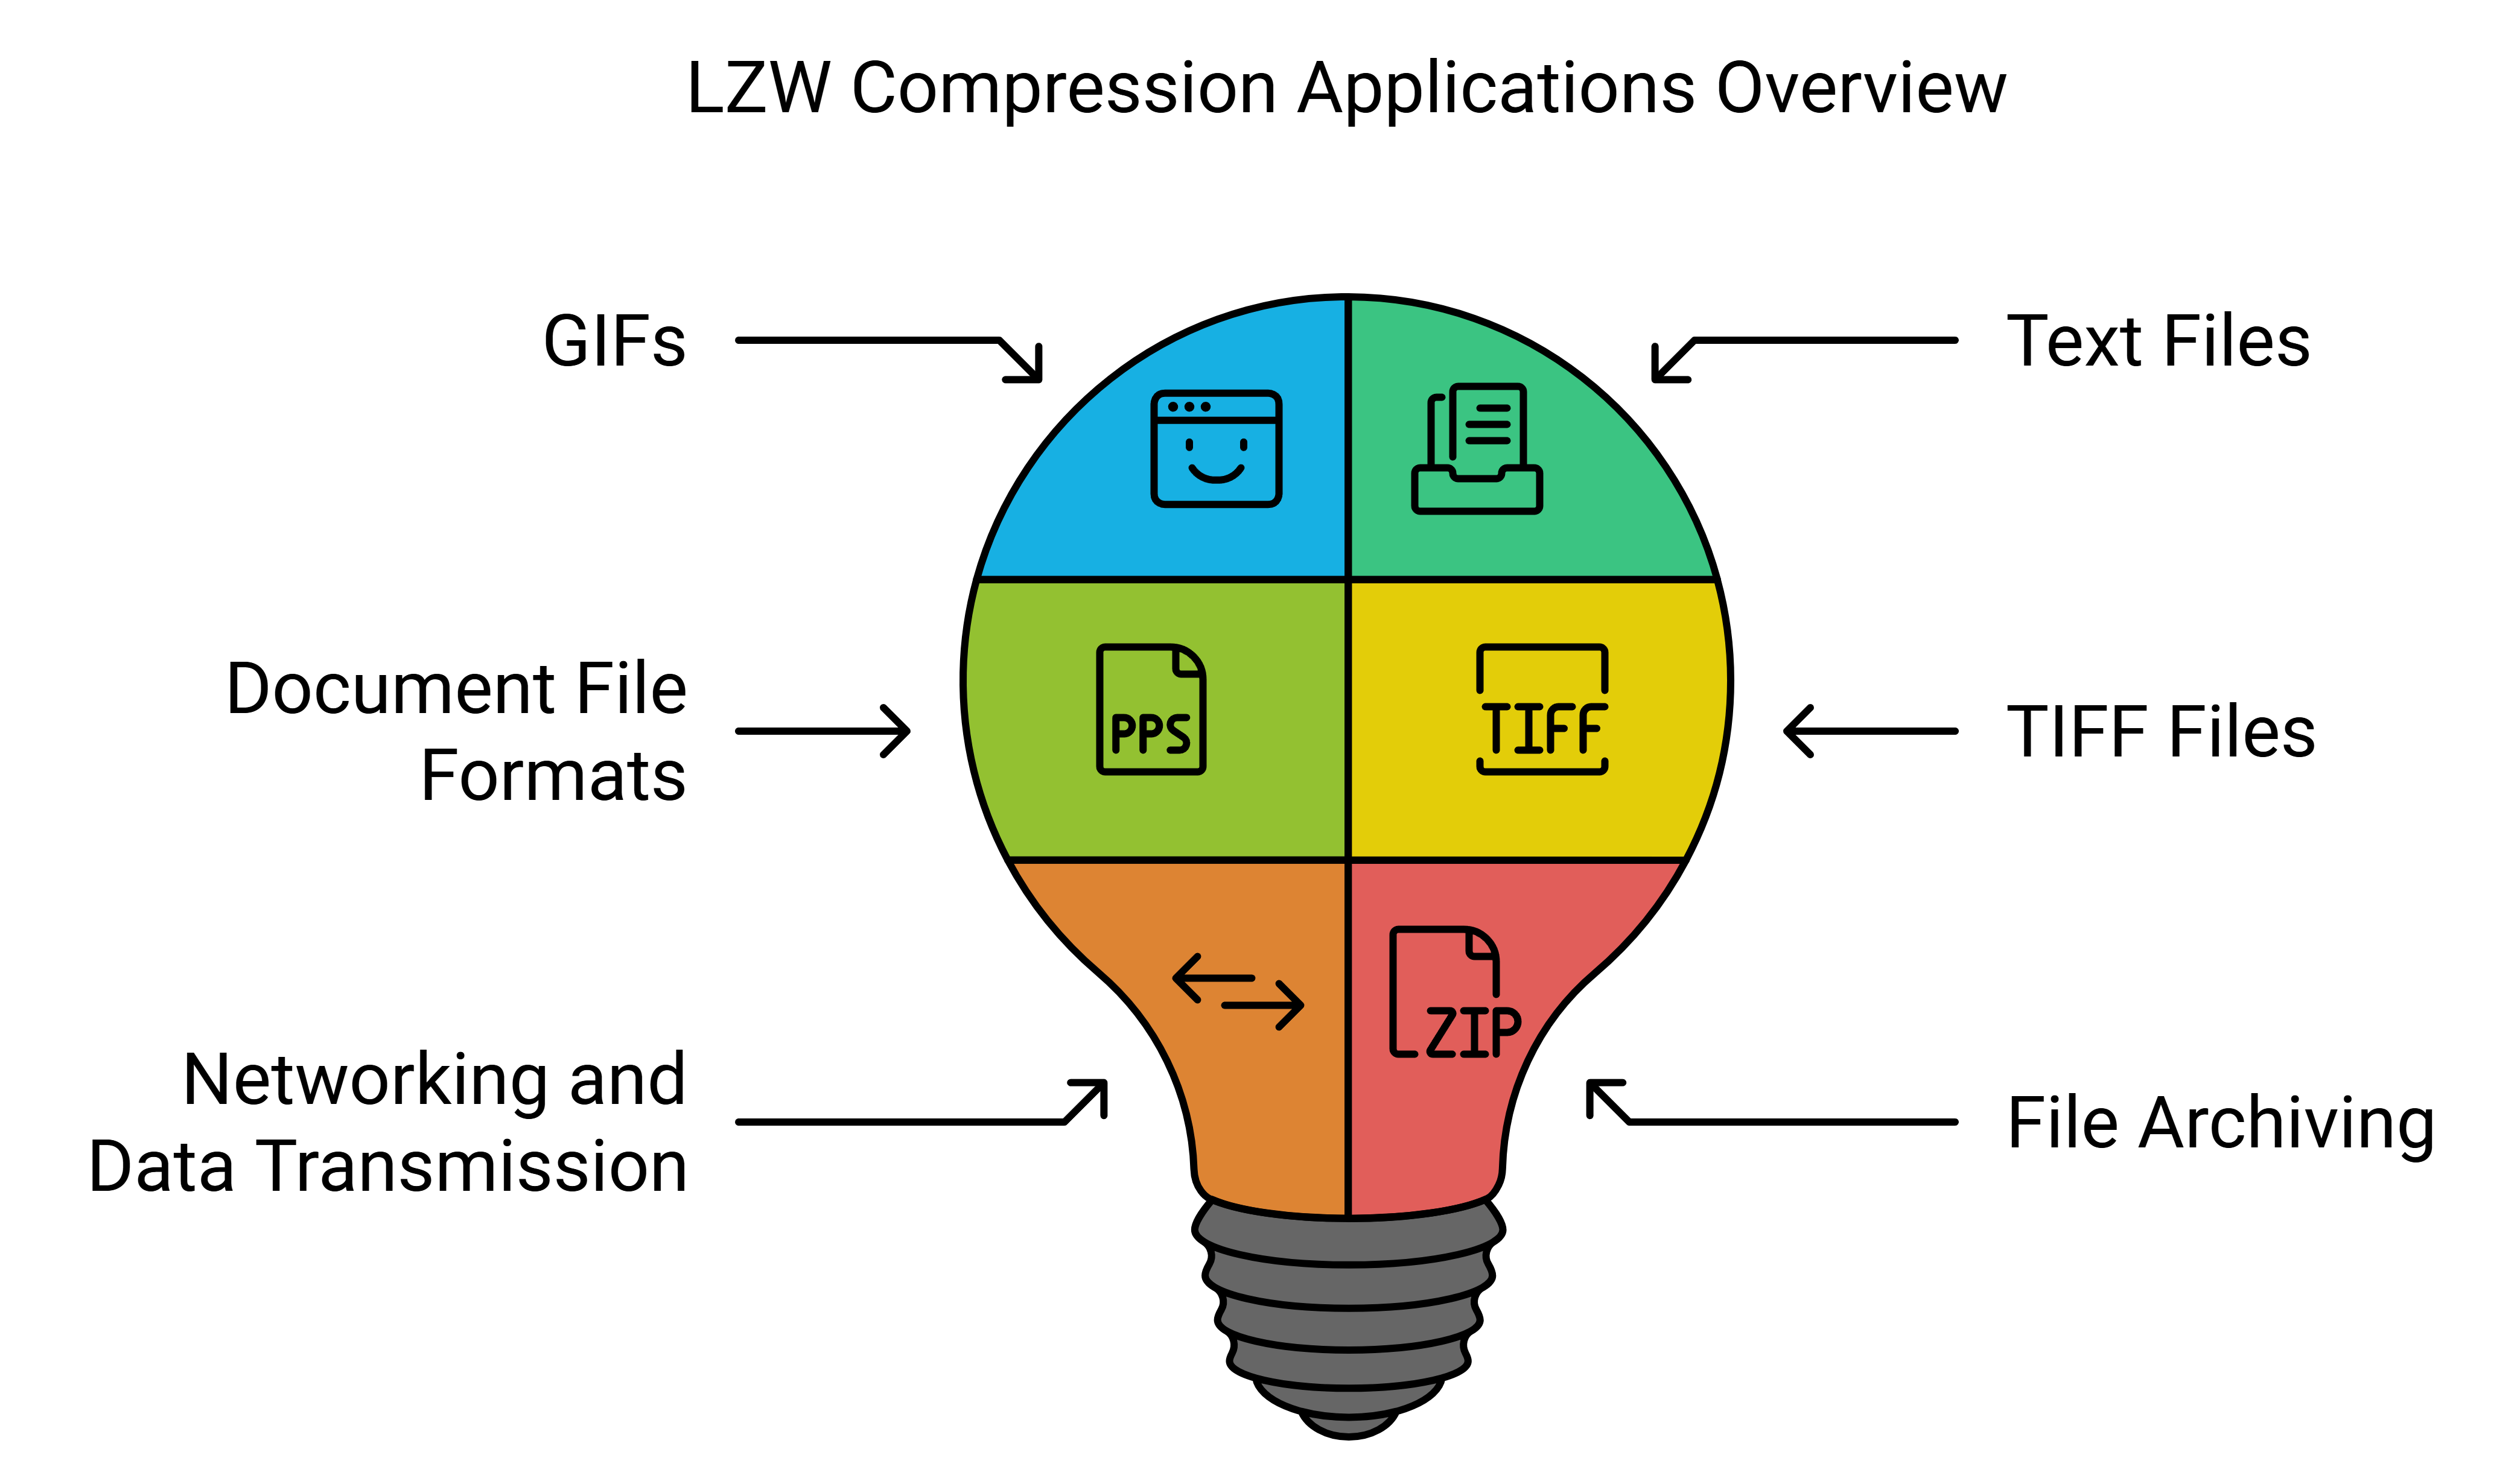
\includegraphics[width=0.8\linewidth]{Figures/application.png}
    \caption{Applications of LZW Compression}
\end{figure}

The LZW compression algorithm is a cornerstone of modern data compression, applied extensively due to its efficiency and reliability. One of its most recognizable applications is in the \textit{GIF (Graphics Interchange Format)}. GIFs utilize LZW compression to minimize file sizes while preserving image quality, enabling quick load times and low bandwidth usage, which are crucial for web graphics and animations.

\vspace{10pt}

In the domain of \textit{text compression}, LZW is highly effective for files with repetitive patterns, such as structured data in XML or JSON formats. By replacing repeating strings with shorter codes, the algorithm significantly reduces file sizes while retaining the ability to reconstruct the original content without any loss. This makes LZW indispensable in archiving and transferring text-based data.

\vspace{10pt}

LZW also plays a pivotal role in \textit{document file formats} like PostScript and PDF. These formats benefit from LZW's ability to optimize file sizes without compromising the integrity of the content, ensuring rapid rendering and efficient storage. This application is particularly valuable in professional publishing and document sharing.

\vspace{10pt}

In addition to GIFs, LZW is used in certain \textit{TIFF (Tagged Image File Format)} files. This is particularly relevant in medical imaging and archival photography, where maintaining high precision is essential. The lossless compression provided by LZW ensures that the quality and integrity of these critical files remain intact.
\vspace{10pt}

LZW's impact extends to \textit{networking and data transmission}. By compressing data before sending it, the algorithm reduces bandwidth requirements and accelerates transfer speeds, making it integral to systems that rely on high-speed communication and efficient resource usage.

\vspace{10pt}

Finally, the influence of LZW can be seen in \textit{file archiving and software packaging tools}. Formats like ZIP have drawn inspiration from LZW’s principles to enable efficient storage and transfer of large datasets and software installations. This reliability and effectiveness in handling large volumes of data have made LZW a foundational component in these technologies.

\vspace{10pt}

These examples demonstrate LZW’s versatility and its ability to address diverse needs, from compressing multimedia files to enhancing network efficiency. The algorithm’s continued relevance is a testament to its robustness and adaptability in modern computing.
